\documentclass[10pt,a4paper]{article}
\usepackage[utf8]{inputenc}
\usepackage{graphicx}
\usepackage{paracol}
\usepackage{geometry}
\usepackage{hyperref}
\usepackage[dvipsnames]{xcolor}
\usepackage{titlesec}
\usepackage{fontawesome}
\usepackage{url}
\usepackage{microtype}
\usepackage{xurl}
\usepackage{tikz}
\usepackage{progressbar}

\geometry{a4paper, margin=0.4in, top=0.4in, bottom=0.4in}

\hypersetup{
    colorlinks=true,
    linkcolor=NavyBlue,
    filecolor=magenta,
    urlcolor=NavyBlue,
}

% Define professional color scheme
\definecolor{primaryblue}{RGB}{41, 128, 185}
\definecolor{darkblue}{RGB}{52, 73, 94}
\definecolor{lightgray}{RGB}{236, 240, 241}
\definecolor{mediumgray}{RGB}{149, 165, 166}
\definecolor{darkgray}{RGB}{44, 62, 80}
\definecolor{accentgreen}{RGB}{39, 174, 96}

% Custom section formatting
\titleformat{\section}{\color{primaryblue}\large\bfseries}{}{0em}{}[\color{primaryblue}\titlerule[1pt]]
\titlespacing*{\section}{0pt}{1.2ex plus 1ex minus .2ex}{1.2ex plus .2ex}

\titleformat{\subsection}{\color{darkblue}\normalsize\bfseries}{}{0em}{}
\titlespacing*{\subsection}{0pt}{1ex plus 1ex minus .2ex}{0.8ex plus .2ex}

\renewcommand{\familydefault}{\sfdefault}

% Skill bar command
\newcommand{\skillbar}[2]{%
    \begin{tikzpicture}[baseline=-0.5ex]
        \fill[lightgray] (0,0) rectangle (3,0.3);
        \fill[primaryblue] (0,0) rectangle (#2*3/5,0.3);
        \node[anchor=west] at (3.2,0.15) {\small #1};
    \end{tikzpicture}%
}

% Language proficiency bar
\newcommand{\langbar}[2]{%
    \begin{tikzpicture}[baseline=-0.5ex]
        \fill[lightgray] (0,0) rectangle (2.5,0.25);
        \fill[accentgreen] (0,0) rectangle (#2*2.5/5,0.25);
        \node[anchor=west] at (2.7,0.125) {\small #1};
    \end{tikzpicture}%
}

\begin{document}

\pagestyle{empty}

% Header section
\begin{center}
    \colorbox{lightgray}{%
        \begin{minipage}{\textwidth}
            \centering
            \vspace{8pt}
            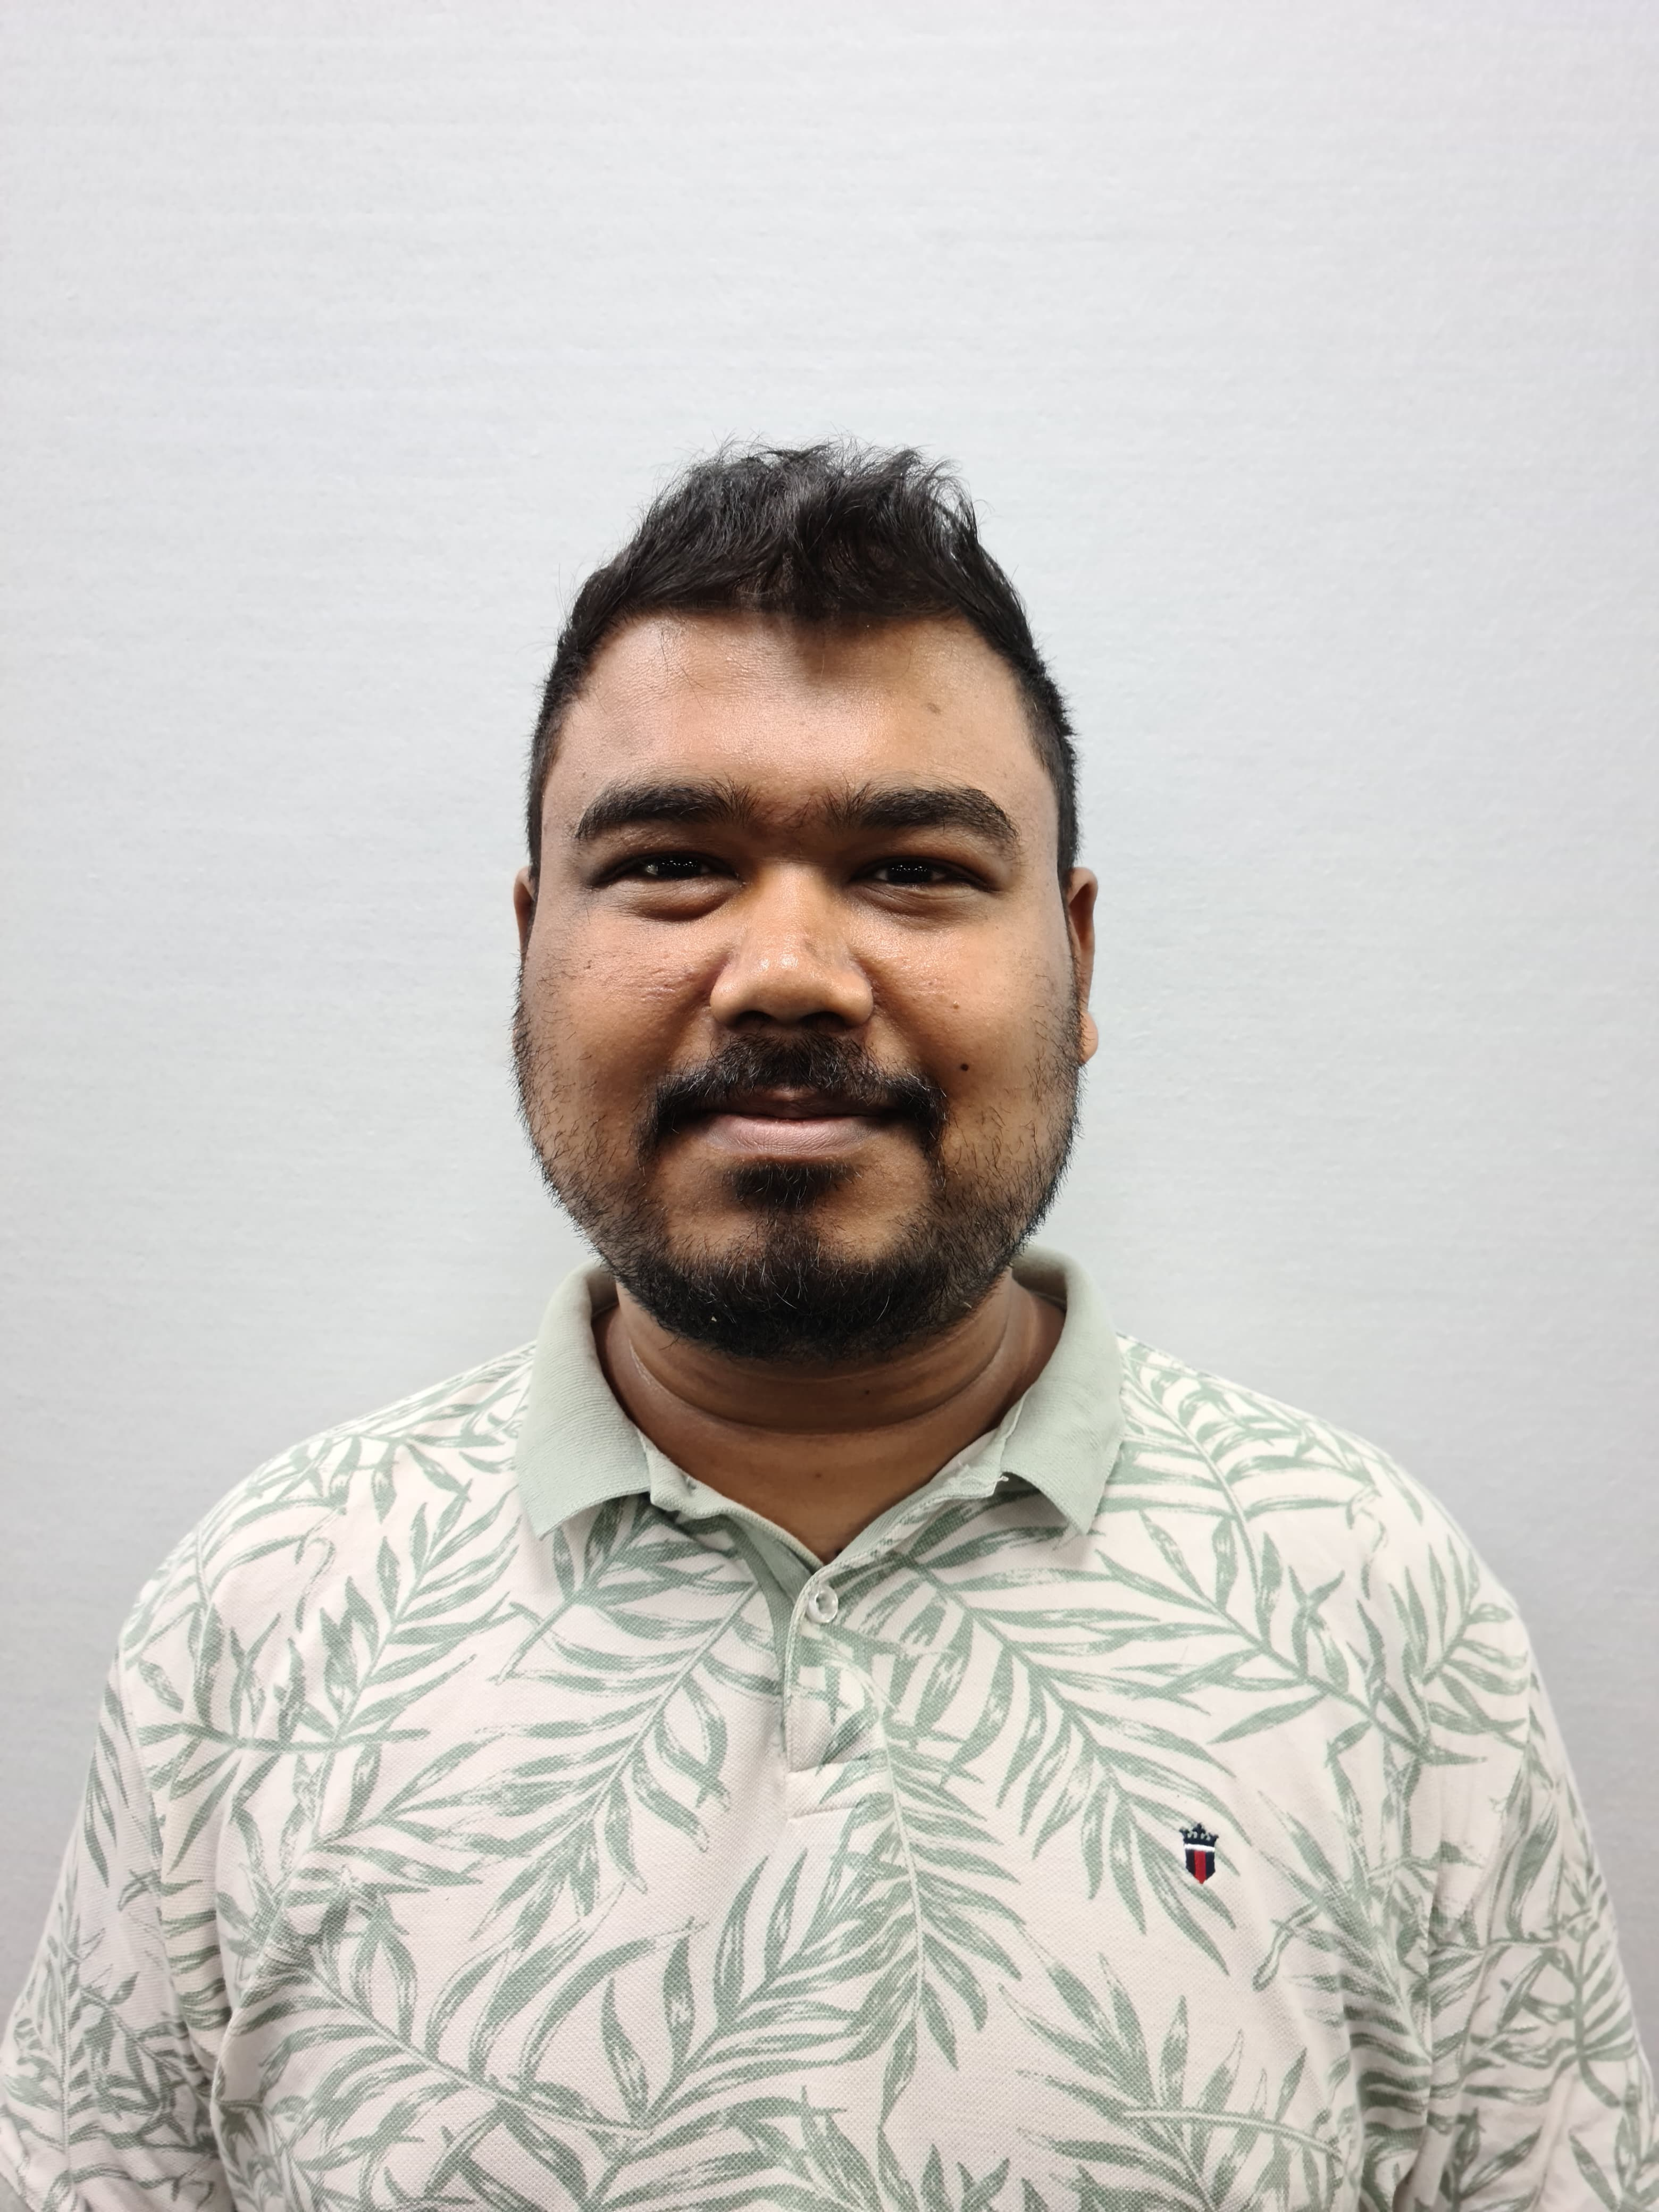
\includegraphics[width=0.08\textwidth,height=0.08\textwidth,keepaspectratio,clip]{passport_photo.jpeg} \\
            \vspace{4mm}
            {\Huge \textbf{\color{darkblue}Biswadeep Baruah}} \\
            \vspace{2mm}
            {\Large \color{primaryblue} Software Developer} \\
            \vspace{2mm}
            {\color{mediumgray} \faMapMarker\ Assam, Gurgaon \quad \faPhone\ +91 8011245653 \quad \faEnvelope\ bswbrh3@gmail.com}
            \vspace{8pt}
        \end{minipage}
    }
\end{center}
\vspace{3mm}

% Two column layout with adjusted column widths
\columnratio{0.32}
\begin{paracol}{2}

% LEFT COLUMN (Narrower)
\begin{leftcolumn}

\section*{\faUser\ PERSONAL INFO}
\textcolor{darkgray}{
\small
\textbf{Address:} \\
Fauzdaripatty b.bora road \\
P.O: Haibargaon \\
Dist.: Nagaon, Assam-782002 \\[2mm]
\textbf{Phone:} +91 7002615821 \\
\textbf{Email:} bswbrh3@gmail.com
}

\vspace{3mm}
\section*{\faCogs\ TECHNICAL SKILLS}
\textcolor{darkgray}{
\small
\skillbar{Python}{5} \\[2mm]
\skillbar{PHP}{4} \\[2mm]
\skillbar{Laravel}{4} \\[2mm]
\skillbar{Flask}{4} \\[2mm]
\skillbar{MySQL}{4} \\[2mm]
\skillbar{MongoDB}{3} \\[2mm]
\skillbar{Git}{4} \\[2mm]
\skillbar{Postman}{4}
}

\vspace{3mm}
\section*{\faGraduationCap\ EDUCATION}
\textcolor{darkgray}{
\small
\textbf{2022 - MTECH} \\
University of Hyderabad \\
\textcolor{primaryblue}{CGPA: 81.30} \\[2mm]

\textbf{2018 - BTECH} \\
Jorhat Engineering College \\
\textcolor{primaryblue}{CGPA: 66.00} \\[2mm]

\textbf{2013 - HSSLC} \\
Vikas Vidyaniketan \\
\textcolor{primaryblue}{Percentage: 81.00} \\[2mm]

\textbf{2011 - HSLC} \\
Christ Jyoti School \\
\textcolor{primaryblue}{Percentage: 69.00}
}

\vspace{3mm}
\section*{\faLanguage\ LANGUAGES}
\textcolor{darkgray}{
\small
\langbar{Assamese}{5} \\[2mm]
\langbar{English}{4} \\[2mm]
\langbar{Hindi}{4}
}

\vspace{3mm}
\section*{\faTrophy\ ACHIEVEMENTS}
\textcolor{darkgray}{
\small
\textbf{2023} Rising Star Award \\
Expand My Business \\[2mm]
\textbf{2011} Anundoram Borooah Award \\[2mm]
\textbf{2008} 37th position \\
Maths Olympiad
}

\vspace{3mm}
\section*{\faHeart\ INTERESTS}
\textcolor{darkgray}{
\small
\faGamepad\ Strategic Gaming \\[1mm]
\faMusic\ Guitar \& Music
}

\vspace{3mm}
\section*{\faGlobe\ SOCIAL}
\textcolor{darkgray}{
\small
\faGithub\ \href{https://github.com/Biswa17}{Biswa17} \\[1mm]
\faLinkedin\ \href{https://linkedin.com/in/biswa-baruah}{Biswa Baruah}
}

\end{leftcolumn}

% RIGHT COLUMN (Wider)
\begin{rightcolumn}

\section*{\faBriefcase\ PROFESSIONAL SUMMARY}
\textcolor{darkgray}{
Highly skilled backend developer with strong proficiency in Python and Laravel, offering over a year of experience in creating efficient and scalable solutions. Proven track record in developing e-commerce platforms, microservices architecture, and API integrations. Seeking challenging opportunities to leverage expertise and contribute to dynamic organizations.
}

\vspace{3mm}
\section*{\faBuilding\ WORK EXPERIENCE}

\subsection*{Backend Developer | Expand My Business \hfill \textcolor{primaryblue}{Oct 2022 – Present}}

\textbf{\color{darkblue}PHP Developer} \hfill \textcolor{mediumgray}{Feb 2023 - Feb 2024}
\textcolor{darkgray}{
\begin{itemize}
    \item \textbf{Snabbcom (Feb 2023 - May 2023):} Developed backend for e-commerce website creation platform using Laravel. Designed RESTful APIs, implemented security measures, and optimized system performance.
    
    \item \textbf{Tata Star Delite \& Star Quik (May 2023 - Nov 2023):} Contributed to live Tata projects using microservice architecture. Integrated Wizzy search services and implemented email/SMS integration with third-party services.
    
    \item \textbf{Socialee E-commerce App (Sept 2023 - Ongoing):} Developed backend for e-commerce app with reel feature. Implemented multi-country, multi-language support (Arabic/English) for Dubai, Riyadh, and India markets. Created unique earning model for content creators.
\end{itemize}
}

\textbf{\color{darkblue}Python Developer} \hfill \textcolor{mediumgray}{Oct 2022 - Feb 2023}
\textcolor{darkgray}{
\begin{itemize}
    \item Developed backend for B2B marketplace connecting vendors and clients across e-commerce, ERP, gaming, and digital marketing verticals. Built scalable features, integrated APIs, and optimized database performance.
\end{itemize}
}

\vspace{3mm}
\section*{\faCode\ KEY PROJECTS}

\textbf{\color{darkblue}Regional Transport Office Vehicle Registration System} \hfill \textcolor{mediumgray}{2016}
\textcolor{darkgray}{
\begin{itemize}
    \item Designed streamlined vehicle registration system for BTech project
    \item Implemented data validation, user authentication, and database management
\end{itemize}
}

\textbf{\color{darkblue}Parallel Programming Optimization} \hfill \textcolor{mediumgray}{2018}
\textcolor{darkgray}{
\begin{itemize}
    \item Enhanced program efficiency using parallel programming techniques
\end{itemize}
}

\textbf{\color{darkblue}Cryptanalysis of Lightweight Block Cipher} \hfill \textcolor{mediumgray}{2021}
\textcolor{darkgray}{
\begin{itemize}
    \item Conducted research on Twine-80 cipher vulnerability
    \item Identified theoretical exploit reducing break time from $2^{80}$ to $2^{78}$
\end{itemize}
}

\vspace{3mm}
\section*{\faWrench\ CORE COMPETENCIES}
\textcolor{darkgray}{
\begin{itemize}
    \item \textbf{Backend Development:} Python, PHP, Laravel, Flask
    \item \textbf{Database Management:} MySQL, MongoDB
    \item \textbf{API Development:} RESTful APIs, Third-party integrations
    \item \textbf{Architecture:} Microservices, Scalable system design
    \item \textbf{Tools \& Technologies:} Git, Postman, Search services integration
    \item \textbf{Specializations:} E-commerce platforms, Multi-language applications
\end{itemize}
}

\end{rightcolumn}
\end{paracol}

\end{document}
